\section{Problem Statement and Goals}
\label{sec:problem}
The aim of the tool is to discover relations in separated datasets (Gene Ontology graph and cluster analysis result tree), visualize and allow interactive selection relations selection.


First step in the program work is loading data and to compute connected components. Data is stored in GML file format. More detailed information about this format and other graph file formats is in the section~\ref{sec:dataset_description}.

Here is program algorithm explanation using sample graphs:
\begin{enumerate}
\item The program visualizes Gene Ontology and cluster analysis result tree. Visualization technic is discussed in the section~\ref{sec:solution}.

\item Interactively select node in the Gene Ontology graph (Figure~\ref{fig:step_1}).

\begin{figure}[h!]
\centering
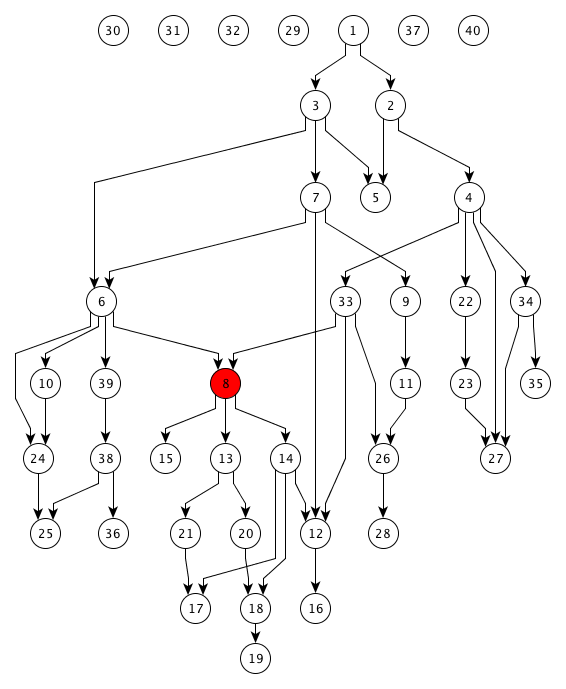
\includegraphics[scale=0.6]{pictures/subgraph_extraction_algorithm_step_1.png}
\caption{Selected node in the Gene Ontology}
\label{fig:step_1}
\end{figure}

\newpage
\item When node is selected in the Gene Ontology program computes all successors (Figure~\ref{fig:step_2}).

\begin{figure}[h!]
\centering
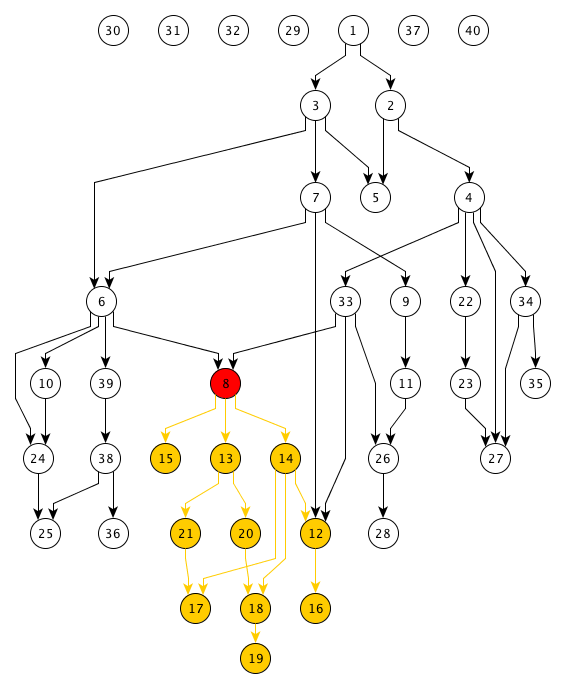
\includegraphics[scale=0.6]{pictures/subgraph_extraction_algorithm_step_2.png}
\caption{Corresponded successors of the selected node}
\label{fig:step_2}
\end{figure}

\newpage
\item Extract leafs from successors (Figure~\ref{fig:step_3}).

\begin{figure}[h!]
\centering
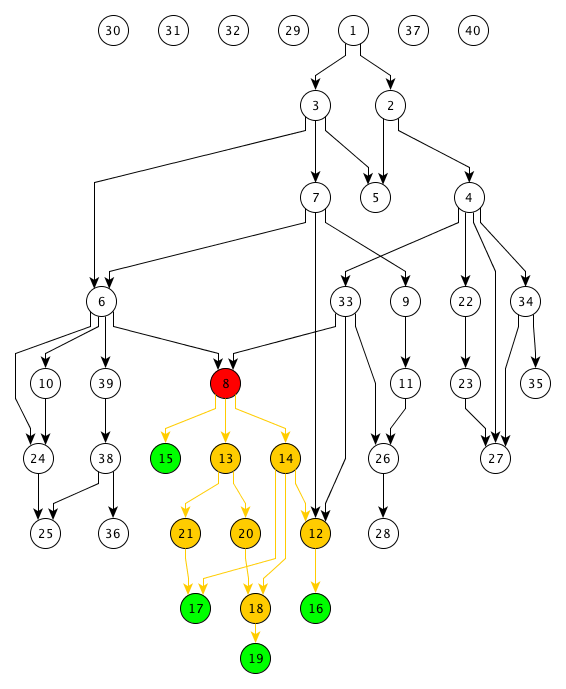
\includegraphics[scale=0.6]{pictures/subgraph_extraction_algorithm_step_3.png}
\caption{Extract leafs}
\label{fig:step_3}
\end{figure}

\newpage
\item Then the program searches corresponded leaves in cluster analysis result tree by label as seen on the Figure~\ref{fig:step_4}.

\begin{figure}[h!]
\centering
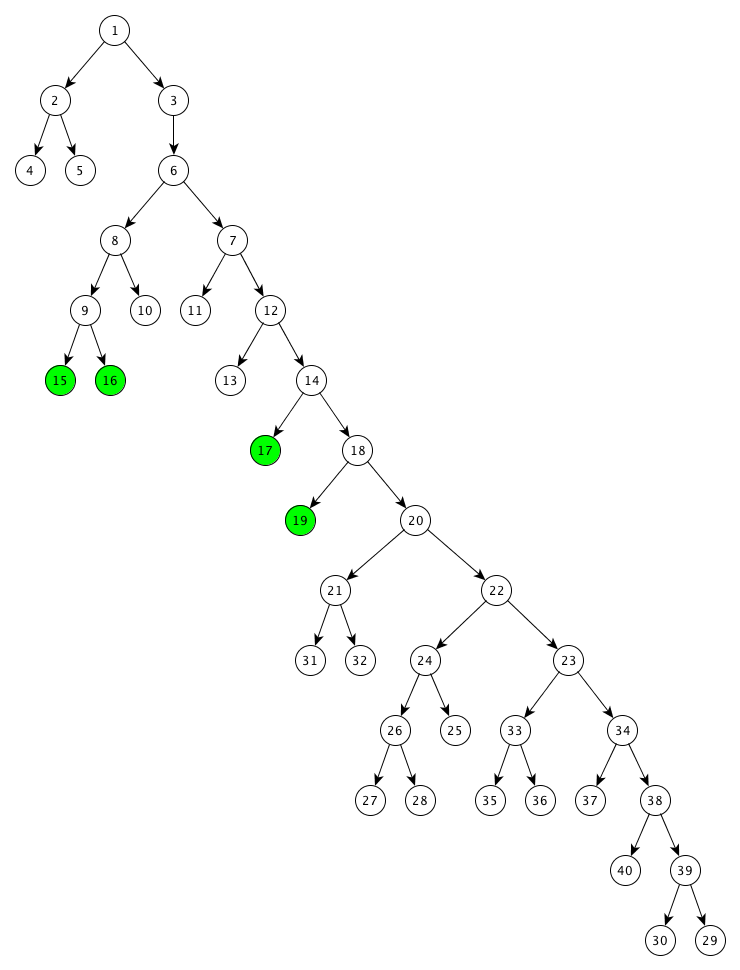
\includegraphics[scale=0.5]{pictures/subgraph_extraction_algorithm_step_4.png}
\caption{Corresponded leaves in the cluster tree}
\label{fig:step_4}
\end{figure}

\newpage
\item For this leaves the program founds root connected to all leaves and extract corresponding sub trees (Figure~\ref{fig:step_5}).

\begin{figure}[h!]
\centering
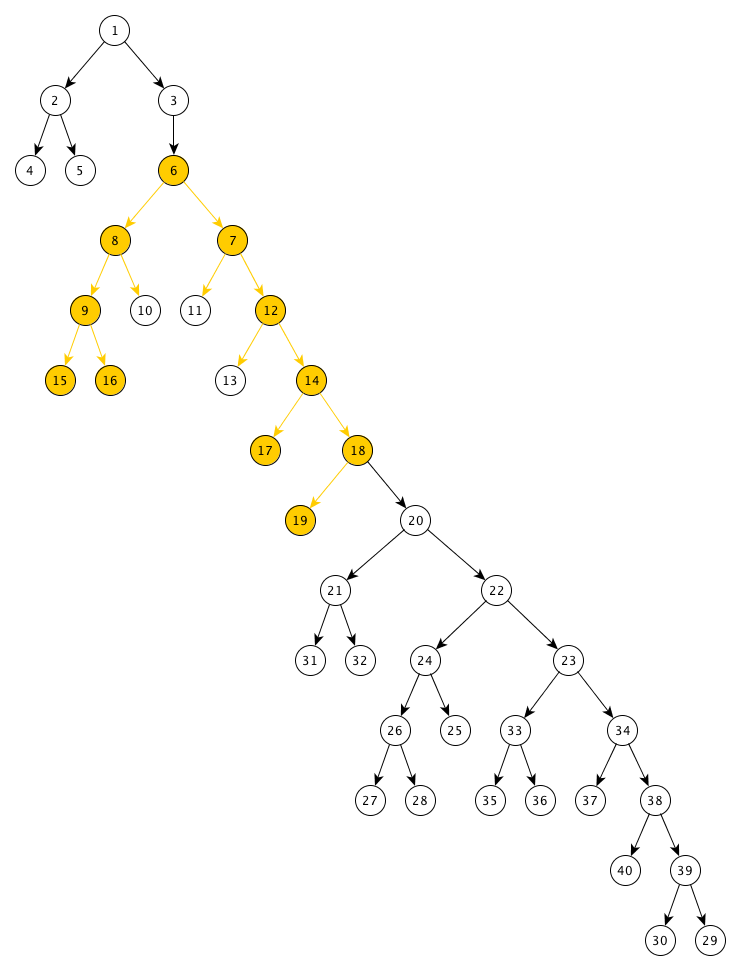
\includegraphics[scale=0.5]{pictures/subgraph_extraction_algorithm_step_5.png}
\caption{Build sub tree}
\label{fig:step_5}
\end{figure}


\item Founded sub tree cached. This sub tree is highlighted in cluster analysis tree.
\end{enumerate}


\subsection{Thesis Collaboration}
There are many datasets for analysis in biology. This work is intended for making a visualization tool for genes and gene relations, in order to help biologists
with their work with genes. This project is result of collaboration between ISOVIS research group (Head: Prof. Dr. Andreas Kerren~\cite{Kerren}) of Linneuniversitetet at V\"axj\"o, Sweden, and Plant Bioinformatics Group (Head: Prof. Dr. Falk Schreiber~\cite{Schreiber}) of Leibniz Institute of Plant Genetics and Crop Plant Research (IPK), Germany.


About the ISOVIS group: "The ISOVIS group mainly focuses on the exploration analysis and visualization of typically large information spaces, for example, in Software Engineering, Geography, or Biology. Another research topic is the use of visualizations in educational software, especially for computer science education. Hereby, we focus on so-called human-centred visualization techniques and approaches:
Human-Centred Visualization combines traditional visualization techniques with the ability of the human visual-brain system and/or the haptic-motoric system to explore and analyse complex data sets comprehensively. This kind of visualization merges several aspects of different research areas, such as Information Visualization, Scientific Visualization, Human-Computer Interaction, Data Mining, Information Design, Graph Drawing, and Computer Graphics. From all sub fields in visualization, we mainly focus on Information Visualization which centres on the visualization of abstract data, e.g., hierarchical, networked, or symbolic information sources, in order to help users understand and analyse such data.


For most practical applications, researchers try to find the best visual representation of the given information. That is the core problem of each visualization but sometimes the seemingly best representation does not suffice if the human information processing and the human capability of information reception are not adequately taken into account. Additionally, these aspects depend on the data to be visualized and on the user's background. While the development of human-centred visualization tools, user abilities and requirements, visualization tasks, tool functions, and visual representations should be equally taken into account. The design of such tools is one of the large challenges of Information Visualization, Software Visualization, and of many application areas, such as the visualization of biological/biochemical or geographical information."~\cite{ISOVIS}


As said on official page of Plant Bioinformatic Group: �The research group focuses on modelling, analysis, simulation and visualisation of biological networks in the context of plant biological problems. Our aim is the development of methods and software tools for the analysis of complex biological networks. Therefore we integrate, process and analyse data from different areas of genome, proteome and
metabolome research and present the results in a user-friendly way. The emphasis is on the linkage of experimental data about expression profiles and metabo-
lite patterns with metabolic and regulatory networks. The data and complex connections are modelled using graphs. We are developing graph (network) analysis and interactive visualisation methods to discover network properties and to make the data easily accessible to the user. A subsequent step is to use the data for the simulation of metabolic and regulatory networks.�~\cite{PBG}


\subsection{Dataset Description}
\label{sec:dataset_description}
Gene Ontology data and cluster analysis results presented as directed graphs. They are stored in separate files in special format -- GML files. GML file format covered in the next section.


GO graph is directed acyclic graph has 10042 vertices and  24155 edges. It has 1 root, 2729 nodes and 7312 leafs (terminal nodes). In the Figure~\ref{fig:yed_GO_vis} showed visualization of the Gene Ontology graph using yEd~\cite{yed} graph editor using Hierarchical layout. It is obviously shows imperfectness of classic visualization of the graphs.


\begin{figure}[h!]
\centering
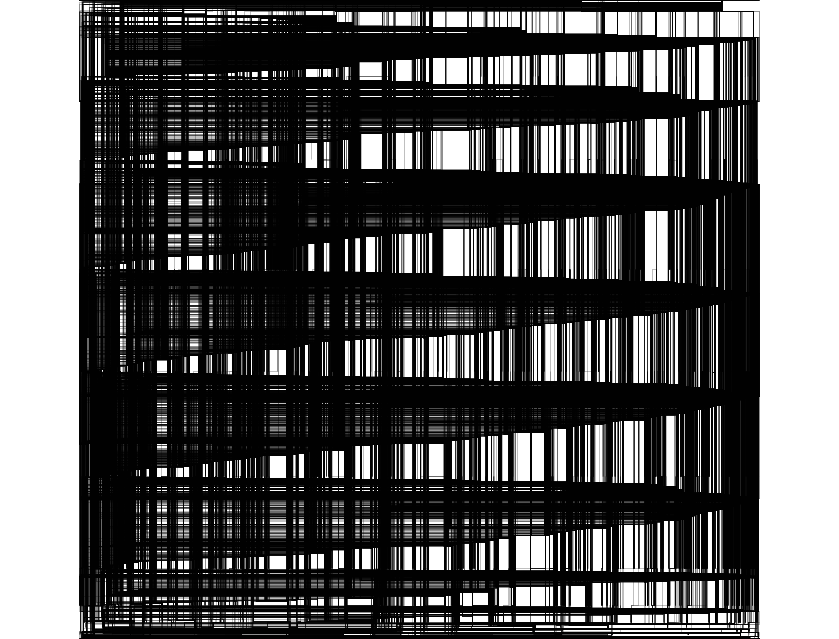
\includegraphics[scale=0.3]{pictures/yEd_GO.png}
\caption{Gene Ontology yEd visualization}
\label{fig:yed_GO_vis}
\end{figure}


Cluster graph is directed binary  tree has 14623 nodes and 14622. Cluster graph as a tree has 1 root, 7310 nodes and 7312 leafs. To get an impression of the graph on the Figure~\ref{fig:Cytoscape_Cluster_1} is visualization of the cluster tree using Cytoscape~\cite{Cytoscape} visualization tool.

\begin{figure}[h!]
\centering
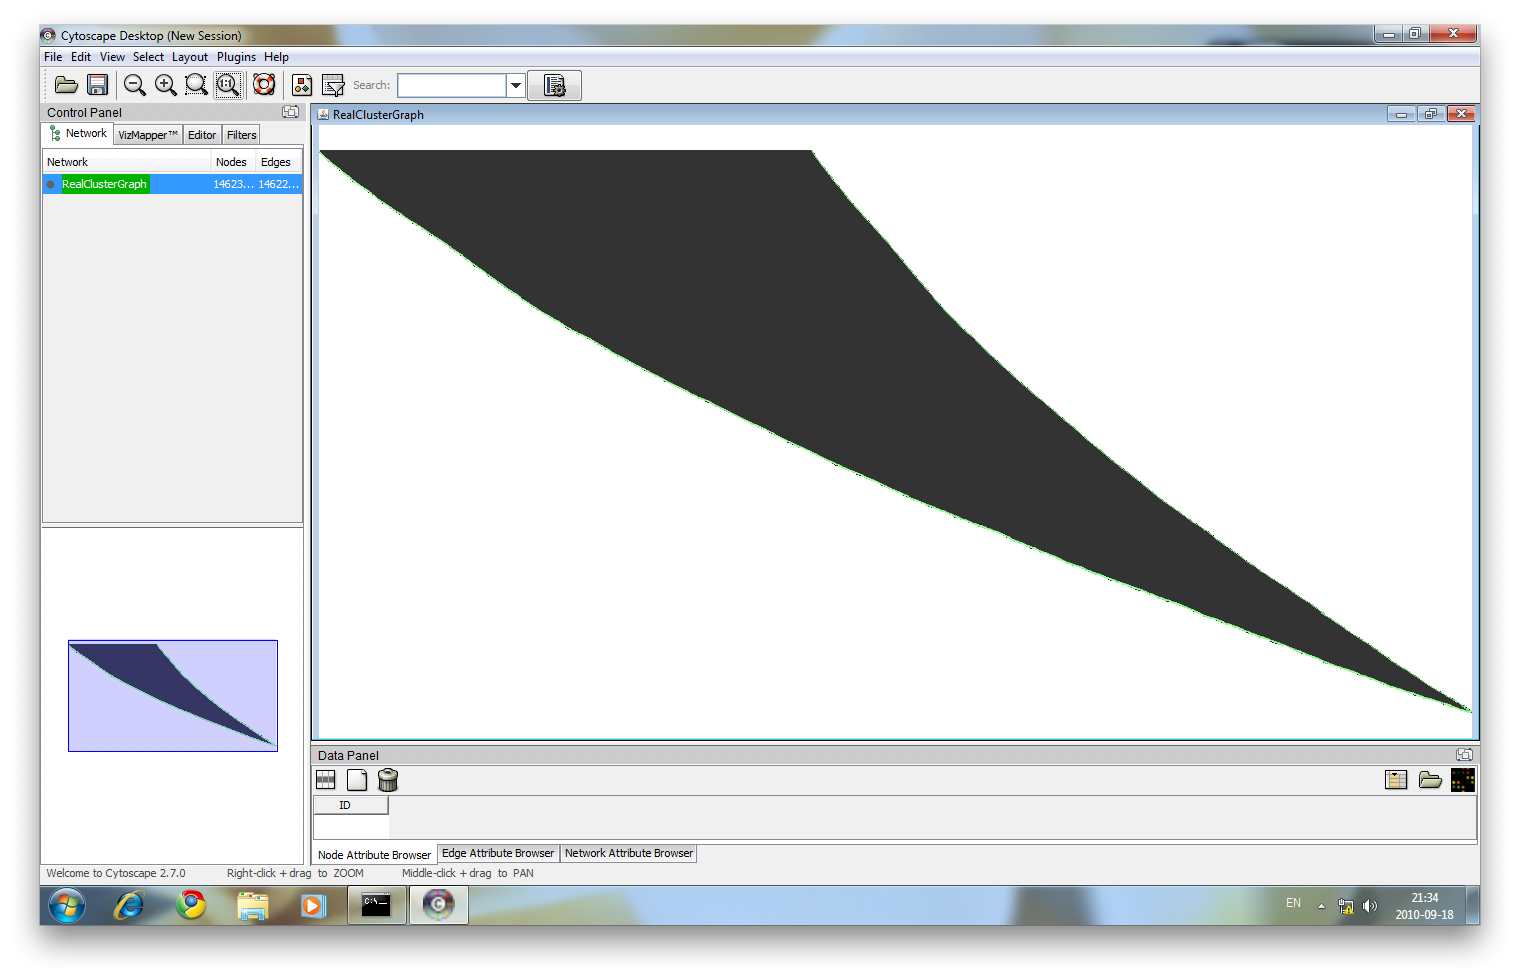
\includegraphics[scale=0.3]{pictures/Cytoscape_cluster_graph_1.png}
\caption{Cluster analysis result tree Cytoscape visualization tool}
\label{fig:Cytoscape_Cluster_1}
\end{figure}

\begin{figure}[h!]
\centering
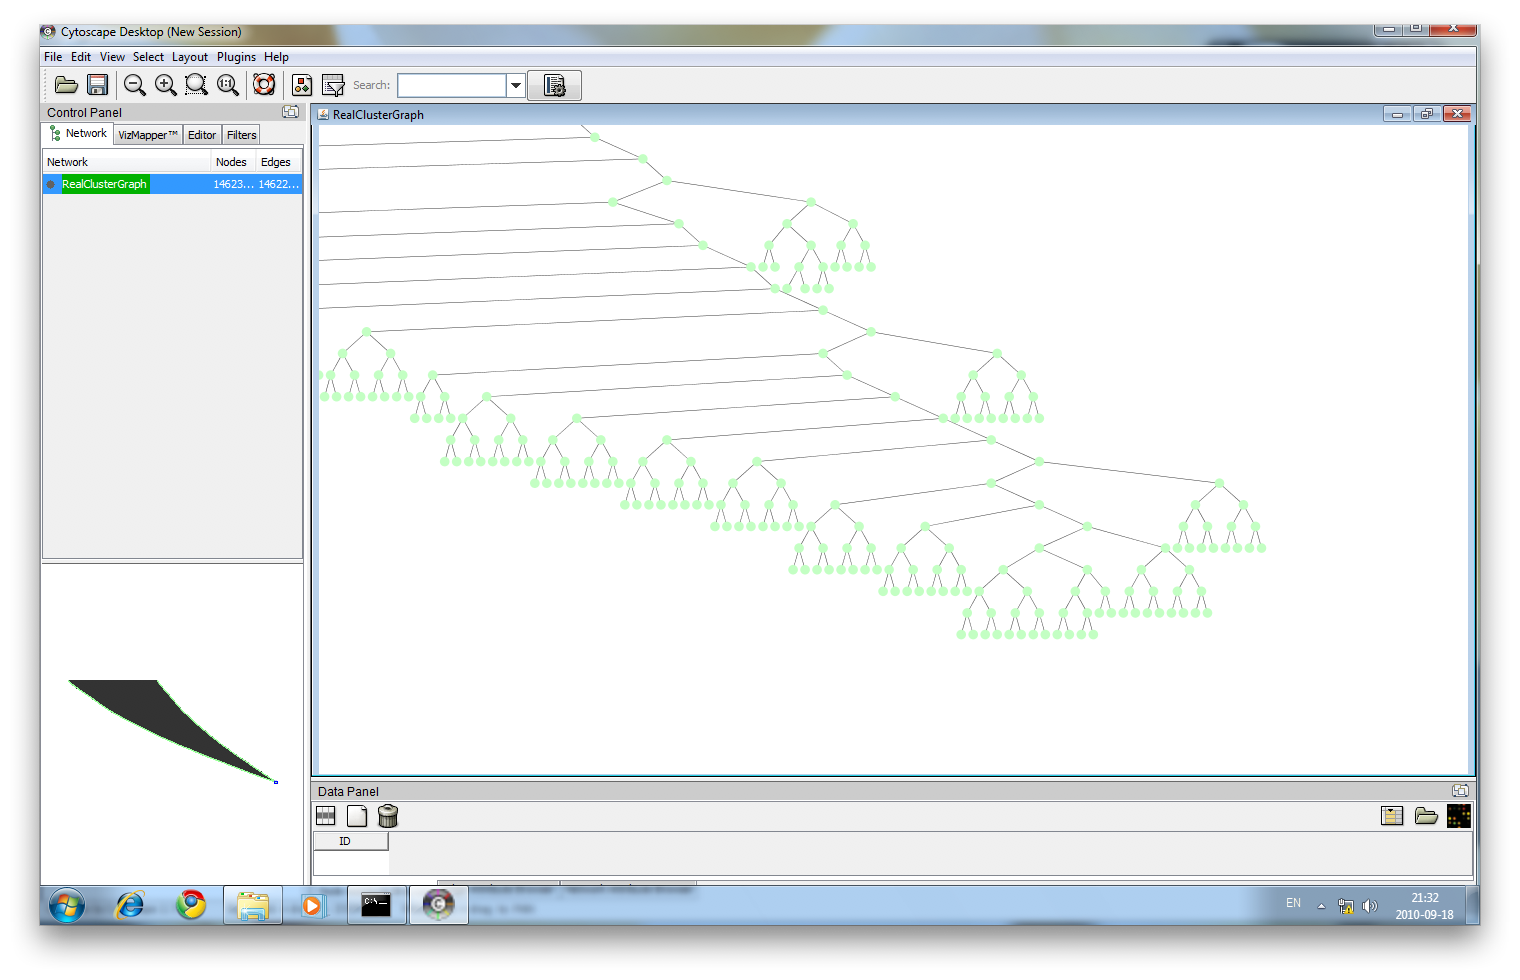
\includegraphics[scale=0.3]{pictures/Cytoscape_cluster_graph_2.png}
\caption{Zoomed cluster analysis result tree}
\label{fig:Cytoscape_Cluster_2}
\end{figure}

Both of two graphs are independent from each other from developer point of view: they have different node ids and edge ids. But they are corresponded by graph node labels -- both of this graphs have same label for terminal (leaf) graph nodes. This property is used in the sub graph extracting algorithm.


The application should work with large quantity of data over tens of thousands that is why performance is one of the main requirements. It is important to give a consideration on optimization.

\subsection{GML Graph File Format}
 "GML, the Graph Modelling Language, is our proposal for a portable file format for graphs. GML's key features are portability, simple syntax, extensibility and flexibility. A GML file consists of a hierarchical key-value lists. Graphs can be annotated with arbitrary data structures. The idea for a common file format was born at the GD'95; this proposal is the outcome of many discussions. GML is the standard file format in the Graphlet~cite{Graphlet} graph editor system. It has been overtaken and adapted by several other systems for drawing graphs."~\cite{GML}


GML format is platform independent, and easy to implement. Furthermore, it has the capability to represent arbitrary data structures, since advanced programs have the need to attach their specific data to nodes and edges. GML is flexible enough that a specific order of declarations is not needed, and that any non-essential data may be omitted. Simple graph is showed in the Listing~\ref{sample_graph_gml}

\begin{center}
	\lstinputlisting[language=xml, tabsize=2, caption={GML description of sample graph}, label={sample_graph_gml}]{graphs/SampleGraph.gml}
\end{center}

In the Figure~\ref{fig:sample_graph_yed_vis} showed manual visualization of the graph using yEd~\cite{yEd}

\begin{figure}[h!]
\centering
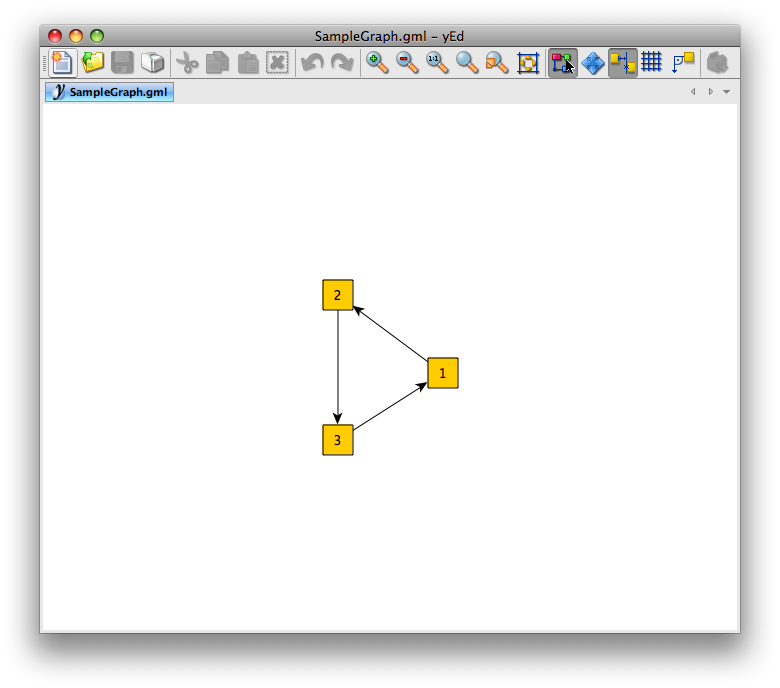
\includegraphics[scale=0.5]{pictures/SampleGraph.png}
\caption{Manual visualization of the sample graph}
\label{fig:sample_graph_yed_vis}
\end{figure}

More complex graph with additional properties and its visualization produced by yEd graph editor is in the Appendix~A and the visualization of this graph showed on the Figure~\ref{fig:yed_graph_vis}

\begin{figure}[h!]
\centering
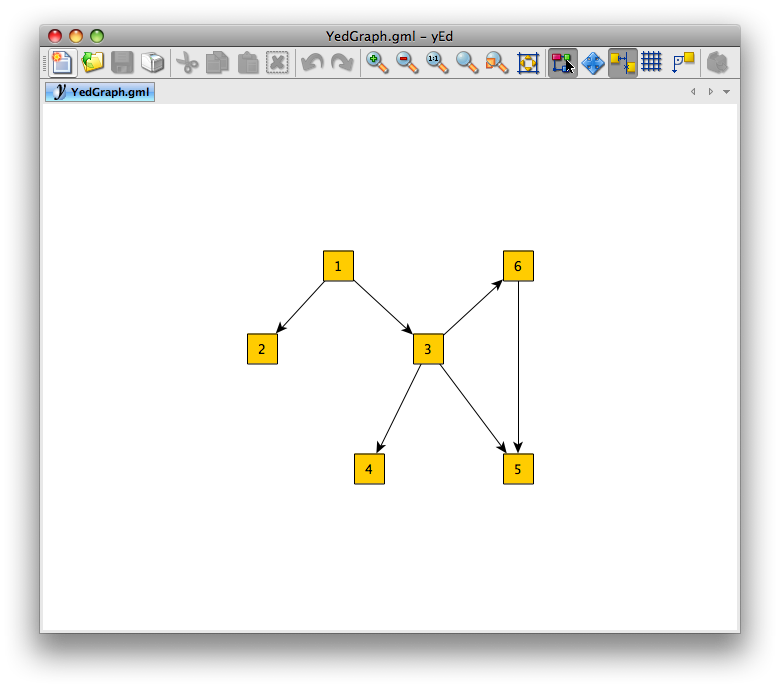
\includegraphics[scale=0.5]{pictures/YedGraph.png}
\caption{Manual visualization of the sample graph}
\label{fig:yed_graph_vis}
\end{figure}

Applications supporting GML~\cite{GML_wiki}

\begin{itemize}
\item Clairlib~\cite{clairlib}, a suite of open-source Perl modules intended to simplify a number of generic tasks in natural language processing (NLP), information retrieval (IR), and network analysis (NA).
\item Cytoscape~\cite{Cytoscape}, an open source bioinformatics software platform for visualizing molecular interaction networks, loads and save previously-constructed interaction networks in GML.
\item NetworkX~\cite{NetworkX}, an open source Python library for studying complex graphs.
\item ocamlgraph\cite{ocamlgraph}, a graph library for OCaml.
\item OGDF\cite{OGDF}, the Open Graph Drawing Framework, an open source C++ library containing implementations of various graph drawing algorithms. The library is self contained; optionally, additional packages like LP-solvers are required for some implementations.
\item Tulip~\cite{Tulip} (software) is a free software in the domain of information visualisation capable of manipulating huge graphs (with more than 1.000.000 elements).
\item yEd~\cite{yed}, a free Java-based graph editor, supports import from and export to GML.
\end{itemize}

\subsection{Other Graph File Formats}

\subsubsection{GraphML}
GraphML is a comprehensive and easy-to-use file format for graphs. It consists of a language core to describe the structural properties of a graph and a flexible extension mechanism to add application-specific data.~\cite{GraphML} Its main features include support of:
\begin{itemize}
\item directed, undirected, and mixed graphs;
\item hyper graphs;
\item hierarchical graphs;
\item graphical representations;
\item references to external data;
\item application-specific attribute data;
\item light-weight parsers;
\end{itemize}

The GraphML document consists of a graphml element and a variety of sub elements: graph, node, edge. In the Figure~\ref{fig:simple_graphml} below is a simple graph. It contains 11 nodes and 12 undirected edges.

\begin{figure}[h!]
\centering
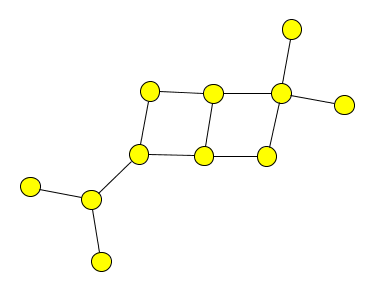
\includegraphics[scale=1.0]{pictures/simple.png}
\caption{A simple graph}
\label{fig:simple_graphml}
\end{figure}


And corresponded graphml file showed in the Listing~\ref{simple_graphml_file}

\begin{center}
\begin{lstlisting} [language=xml, tabsize=2, caption={Simple graphml file},label=simple_graphml_file]
<graphml>
  <graph id="G" edgedefault="undirected">
    <node id="n0"/>
    <node id="n1"/>
    <node id="n2"/>
    <node id="n3"/>
    <node id="n4"/>
    <node id="n5"/>
    <node id="n6"/>
    <node id="n7"/>
    <node id="n8"/>
    <node id="n9"/>
    <node id="n10"/>
    <edge source="n0" target="n2"/>
    <edge source="n1" target="n2"/>
    <edge source="n2" target="n3"/>
    <edge source="n3" target="n5"/>
    <edge source="n3" target="n4"/>
    <edge source="n4" target="n6"/>
    <edge source="n6" target="n5"/>
    <edge source="n5" target="n7"/>
    <edge source="n6" target="n8"/>
    <edge source="n8" target="n7"/>
    <edge source="n8" target="n9"/>
    <edge source="n8" target="n10"/>
  </graph>
</graphml>
\end{lstlisting}
\end{center}

\subsubsection{DOT graph file format}
"DOT is a plain text graph description language. It is a simple way of describing graphs that both humans and computer programs can use. DOT graphs are typically files that end with the .gv (or .dot) extension.


At its simplest, DOT can be used to describe an undirected graph. An undirected graph shows simple relations between objects, such as friendship between people. The graph keyword is used to begin a new graph, and nodes are described within curly braces. A double-hyphen (\textendash \textendash) is used to show relations between the nodes."~\cite{DOT}

\begin{center}
\begin{lstlisting} [language=C, tabsize=2, caption={DOT file format: undirected graph}]
graph graphname {
     a - - b - - c;
     b - - d;
}
\end{lstlisting}
\end{center}

"Similar to undirected graphs, DOT can describe directed graphs, such as flowcharts and dependency trees. The syntax is the same as for undirected graphs, except the digraph keyword is used to begin the graph, and an arrow ($->$) is used to show relationships between nodes."~\cite{DOT}

\begin{center}
\begin{lstlisting} [language=C, tabsize=2, caption={DOT file format: directed graph}]
graph graphname {
     a -> b -> c;
     b -> d;
}
\end{lstlisting}
\end{center}

Visual representation of both graphs showed in the Figure~\ref{fig:dot_graphs} below.

\begin{figure}[h!]
\centering
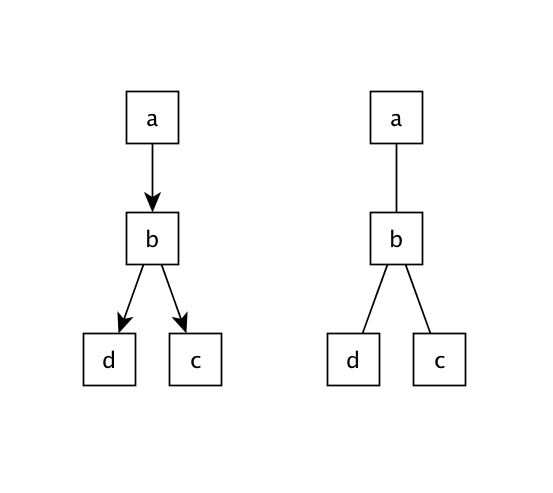
\includegraphics[scale=0.3]{pictures/dot_graph.png}
\caption{Directed and undirected graphs}
\label{fig:dot_graphs}
\end{figure}

\subsubsection{DGML}
DGML is an XML-based file format for directed graphs. Here is what a simple directed graph with three nodes and two links between them looks like

\begin{center}
\begin{lstlisting} [language=XML, tabsize=2, caption={DGML file format}]
<?xml version='1.0' encoding='utf-8'?>
<DirectedGraph xmlns="http://schemas.microsoft.com/vs/2009/dgml">
  <Nodes>
    <Node Id="a" Label="a" Size="10" />
    <Node Id="b" Background="#FF008080" Label="b" />
    <Node Id="c" Label="c" Start="2010-06-10" />
  </Nodes>
  <Links>
    <Link Source="a" Target="b" />
    <Link Source="a" Target="c" />
  </Links>
  <Properties>
    <Property Id="Background" Label="Background" DataType="Brush" />
    <Property Id="Label" Label="Label" DataType="String" />
    <Property Id="Size" DataType="String" />
    <Property Id="Start" DataType="DateTime" />
  </Properties>
</DirectedGraph>
\end{lstlisting}
\end{center}

The complete XSD schema for DGML is available at \url{http://schemas.microsoft.com/vs/2009/dgml/}. DGML not only allows describing nodes and links in a graph, but also annotating those nodes and links with any user defined property and/or category.

\subsubsection{GXL}
"GXL (Graph eXchange Language) is a standard format for exchanging graph-based data. It is the culmination of a cooperative effort among an international group of researchers from disparate areas, including software reengineering and graph transformation. Researchers and tool builders have had a growing interest in comparing and combining approaches to their respective problems and leveraging each other's results. These collaborations provide lessons learned that are critical to advancing the maturity of the discipline. A standard exchange format for data facilitates tool interoperability and allows them to use a "best of breed" approach when building a workbench.


Interoperability is the challenge of enabling tools from different suppliers to work together. Wasserman [1] describes a taxonomy with five types of interoperability: platform, presentation, data, control, and process. Another model from Earl has three levels: control, user interface, and data. Data interoperability appears in both of them.


Data interoperability requires the data to be compatible both syntactically and semantically. In other words, tools need to agree on both the format and the meaning of this data. The graph-based data model of GXL can be used to represent both instance data and schemas.


Thus, GXL provides a standardized notation for exchanging instance data (graphs) including their structure (graph schemas). Both instance and schema graphs are encoded using the same XML (eXtensible Markup Language) DTD (Document Type Definition). While these schema graphs do not provide semantics, they serve as a basis for users to agree upon semantics. This feature is important because it helps tools and researchers communicate about the assumptions inherent in their approaches. This increased mutual understanding is a critical step in building on each other's work to increase the impact of research results.


In addition to being a generic format for representing graph structures, GXL is also suitable for object-relational data. Consequently, GXL can be used to represent data from a wider range of applications, including as data repositories and fact bases from reengineering tools."~\cite{GXL}

\subsubsection{SVG}
"SVG has been in development since 1999 by a group of companies within the W3C after the competing standards Precision Graphics Markup Language (PGML) � developed from Adobe's PostScript � and Vector Markup Language (VML) � developed from Microsoft's RTF � were submitted to W3C in 1998. SVG drew on experience from the designs of both those formats.


SVG allows three types of graphic objects:
\begin{itemize}
\item Vector graphics
\item Raster graphics
\item Text
\end{itemize}

Graphical objects, including PNG and JPEG raster images, can be grouped, styled, transformed, and composited into previously rendered objects. SVG does not directly support z-indices[5] that separate drawing order from document order for overlapping objects, unlike some other vector mark up languages like VML. Text can be in any XML name space suitable to the application, which enhances search ability and accessibility of the SVG graphics. The feature set includes nested transformations, clipping paths, alpha masks, filter effects, template objects and extensibility.


Since 2001, the SVG specification has been updated to version 1.1 (current Recommendation) and 1.2 (still a Working Draft). The SVG Mobile Recommendation introduced two simplified profiles of SVG 1.1, SVG Basic and SVG Tiny, meant for devices with reduced computational and display capabilities. SVG Tiny later became an autonomous Recommendation (current version 1.2) and the basis for SVG 1.2. In addition to these variants and profiles, the SVG Print specification (still a Working Draft) contains guidelines for printable SVG 1.2 and SVG Tiny 1.2 documents.
The Canvas element in HTML 5 provides an approach to rendering dynamic graphics in HTML that's procedural rather than declarative: instead of specifying the shapes to draw in XML, the author executes drawing commands from a script. Canvas doesn't allow for static rendering, and drawn elements are not identifiable in a DOM-like way."~\cite{SVG}
